\documentclass[]{article}
\usepackage{graphicx} % Required for inserting images
\usepackage{hyperref}
\usepackage{tikz}
\usepackage{amsmath}

\newcommand{\pderiv}[2]{\frac{\partial #1}{\partial #2}}

\title{Research Log}
\author{Colin Flanagan}
\date{August 2025}

\begin{document}

\maketitle

\section{8/26/25 - Brainstorming}
Kaggle competitions\\
No time scale forecasting so any regression vs time is a no\\
Want a classifier of some kind
\begin{enumerate}
    \item Just the basics digit/letter classifier\\
    \item 
\end{enumerate}
Sources on neural nets
\url{https://scikit-learn.org/stable/modules/neural_networks_supervised.html}\\
\url{https://scikit-learn/stable/modules/sgd.html}\\
\url{https://www.tensorflow.org/neural_structured_learning}

\section{8/28/25 - Brainstorming}
Video on coding/ the cs view\\
\url{https://www.youtube.com/watch?v=u5GAVdLQyIg}\\
\\
Good video on gradient descent\\
\url{https://www.youtube.com/watch?v=sDv4f4s2SB8}\\
\\
\url{https://en.wikipedia.org/w/index.php?title=Backpropagation&oldid=1296531871}\\
\url{https://en.wikipedia.org/w/index.php?title=Multilayer_perceptron&oldid=1290081276}\\
\url{https://en.wikipedia.org/w/index.php?title=Stochastic_gradient_descent&oldid=1295784793#Adam}\\
\\
Calculations\\
\url{https://medium.com/coinmonks/the-mathematics-of-neural-network-60a112dd3e05}\\

\section{9/4/25 - Forward and Backpropagation Write Up}
\subsection{Introduction}
Machine learning is not coming to find John Connor, rather it is a sophisticated vector and calculus algorithm designed to minimize the error in the algorithm's guess vs the actual outputs of a problem. To start the example let us use two vectors to begin our example. Let $\vec{a^0}$ be the vector of inputs, let $\vec{a^2}$ be the vector of our machine learning algorithms output, and let $\hat{y}$ be the vector of actual outputs.

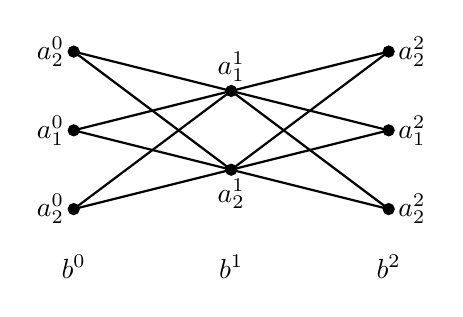
\begin{tikzpicture}

\filldraw[black] (0,0) circle (2pt) node[anchor=east]{$a^{0}_1$};
\filldraw[black] (0,1) circle (2pt) node[anchor=east]{$a^{0}_2$};
\filldraw[black] (0,-1) circle (2pt) node[anchor=east]{$a^{0}_2$};

\filldraw[black] (0,-2) circle (0pt) node[anchor=south]{$b^0$};
\filldraw[black] (2,-2) circle (0pt) node[anchor=south]{$b^1$};
\filldraw[black] (4,-2) circle (0pt) node[anchor=south]{$b^2$};

\filldraw[black] (2,0.5) circle (2pt) node[anchor=south]{$a^{1}_1$};
\draw[black, thick] (0,0) -- (2,0.5);
\draw[black, thick] (0,1) -- (2,0.5);
\draw[black, thick] (0,-1) -- (2,0.5);
\filldraw[black] (2,-0.5) circle (2pt)
node[anchor=north]{$a^{1}_2$};
\draw[black, thick] (0,0) -- (2,-0.5);
\draw[black, thick] (0,1) -- (2,-0.5);
\draw[black, thick] (0,-1) -- (2,-0.5);

\filldraw[black] (4,0) circle (2pt) node[anchor=west]{$a^{2}_1$};
\draw[black, thick] (2,0.5) -- (4,0);
\draw[black, thick] (2,-0.5) -- (4,0);
\filldraw[black] (4,1) circle (2pt) node[anchor=west]{$a^{2}_2$};
\draw[black, thick] (2,0.5) -- (4,1);
\draw[black, thick] (2,-0.5) -- (4,1);
\filldraw[black] (4,-1) circle (2pt) node[anchor=west]{$a^{2}_2$};
\draw[black, thick] (2,0.5) -- (4,-1);
\draw[black, thick] (2,-0.5) -- (4,-1);

\end{tikzpicture}

\begin{align*}
    \vec{a}^0 = \begin{bmatrix}a_{1}^{0}\\a_{2}^{0}\\a_{3}^{0}\end{bmatrix},\vec{a}^2 = \begin{bmatrix}
        a_{1}^{2}\\a_{2}^{2}\\a_{3}^{2}
    \end{bmatrix}\text{and }\hat{y} = \begin{bmatrix}y_1\\y_2\\y_3\end{bmatrix}, 
\end{align*}
\subsection{Forward Propagation}
Patrick Section
\subsection{Backward Propagation}
To start talking about how back propagation works we need to talk about what it is. When a neural network makes its initial guess given a set of inputs, the model needs a way to correct itself if its poorly guessing (common). The strategy to do this is gradient descent or stochastic gradient descent where you calculate the rates of change of the cost function with respect to all the weights and biases. The gradient is a large vector composed of the partial derivative of the cost function with respect to each variable. One way to calculate these derivatives while saving computing power is to use a method called back propagation. To get a look at the way this works let us look at an image of what the gradient represents mathematically. 
\begin{equation}
    \nabla C = \begin{bmatrix}\frac{\partial C}{\partial w^1}\\\frac{\partial C}{\partial b^1}\\\frac{\partial C}{\partial w^2}\\\frac{\partial C}{\partial b^2}\\...\\\frac{\partial C}{\partial w^L}\\\frac{\partial C}{\partial b^L}\label{gradient
    }\end{bmatrix}
\end{equation}
This is what we want to solve for so that we can multiply this vector by our learning rate and adjust the weights and biases in the network to minimize the cost function. In this form it is clear that we are looking to solve for \[\frac{\partial C}{\partial w^L} \text{ and }\frac{\partial C}{\partial b^L}\] or the rate of change with respect to each weight, and each bias. From the chain rule we know that 
\[\frac{d}{dx} = \frac{d}{dy}\frac{dy}{dx}\]
and backpropagation is the method of applying the chain rule to solve for those two partials with derivatives that can be easily calculated rather than calculating new derivatives at each step or calculating a giant derivative. To begin, let us quickly remind ourselves of how how each step of forward propogation is calculated.
\begin{align*}
    \vec{a}^L &= \sigma\left(\vec{z}^L\right)\\
    \vec{z}^L &= W^L\left(\vec{a}^{L-1}\right) + b^L\\
    \sigma &= \text{relu} = \text{max}(0,x)\\
    \vec{a}^{L-1} &= \sigma\left(\vec{z}^L\right)\\
    \vec{z}^{L-1} &= W^{L-1}\left(\vec{a}^{L-2}\right) + b^{L-1}\\
\end{align*}
So in context, this means that the activations, $\vec{a}^L$, for a given layer are given by the activation function, $\sigma$, Rectified Linear Unit function which outputs the max of 0 and the input for the weighted sum function $\vec{z}^L$ . The function $z^L$ is the weighted sum function which takes an input vector, multiplies that by the weight matrix and add the basis vector. To truly see what we need to solve for and how to apply the chain rule, lets look at the cost function, Categorical Cross Entryopy,
\begin{align}
    C = \sum_{i}^{n}\vec{a}^2_i\cdot\text{ln}(\hat{y}_i)
\end{align}
So the sum of the guess times the natural log of the actual output. Let us start with the this partial we need to solve for
\begin{align}
    \frac{\partial{C}}{\partial{b^L}}\\
    \text{or for our case}\\
    \frac{\partial{C}}{\partial{b^2}}
\end{align}
Immediate inspection, reveals that the cost function does not have the basis vector built into it, you would need to do recursion to find it, this is where back propogation saves us. Looking at our partial derivative we need to take it with respect to the basis, so we need to look for a function with $b^L$ in it. That would be $z^L$. So we need to calculate
\begin{align}
    \frac{\partial{z^L}}{\partial{b^L}}
\end{align}
following the chain rule we need to get rid of $z^L$ need another derivative with that in the bottom. And $a^L$ can be taken with respect to $z^L$. Looking at our cost function we can then eliminate the $a^L$.
\begin{align}
    \pderiv{z^L}{b^L} \cdot \pderiv{a^L}{z^L} \cdot \pderiv{C}{a^L}
\end{align}
plugging in our numbers we get this formula.
\begin{align}
    \pderiv{C}{b^2}=\pderiv{z^2}{b^2} \cdot \pderiv{a^2}{z^2} \cdot \pderiv{C}{a^2}
\end{align}

\section{9/26/25 - Digit Recognizer}
Worked and completed what I think is one layer and step of the forward proposition step. Basically all the inputs and they get transformed into some number.

\section{9/30/25 - Digit Recognizer}
Continued working on digit recognizer NN. Worked on matrix multiplication and re familiarizing with numpy. 

\section{10/2/25 - Digit Recognizer}
Continued working on digit recognizer NN. Worked on matrix multiplication and re familiarizing with numpy. 

\section{10/7/25 - Digit Recognizer}
Finished matrix multiplication, worked on soft max.

\section{10/9/25 - Digit Recognizer}
Continued working softmax issues. 

\section{10/11/25 - Digit Recognizer}
Started Beamer slides and updated my research log. I think its also wise to include the commit history from my GitHub page so that all the history of my edits is available\\
https://github.com/flanaganc04/My-own-Neural-Net/commits/main/
\end{document}
